%%%%%%%%%%%%%%%%%%%%%%%%%%%%%%%%%%%%%%%%%
% Beamer Presentation
% LaTeX Template
% Version 1.0 (10/11/12)
%
% This template has been downloaded from:
% http://www.LaTeXTemplates.com
%
% License:
% CC BY-NC-SA 3.0 (http://creativecommons.org/licenses/by-nc-sa/3.0/)
%
%%%%%%%%%%%%%%%%%%%%%%%%%%%%%%%%%%%%%%%%%

%----------------------------------------------------------------------------------------
%	PACKAGES AND THEMES
%----------------------------------------------------------------------------------------

\documentclass{beamer}

\mode<presentation> {

% The Beamer class comes with a number of default slide themes
% which change the colors and layouts of slides. Below this is a list
% of all the themes, uncomment each in turn to see what they look like.

%\usetheme{default}
%\usetheme{AnnArbor}
%\usetheme{Antibes}
%\usetheme{Bergen}
%\usetheme{Berkeley}
%\usetheme{Berlin}
%\usetheme{Boadilla}
%\usetheme{CambridgeUS}
%\usetheme{Copenhagen}
%\usetheme{Darmstadt}
%\usetheme{Dresden}
%\usetheme{Frankfurt}
%\usetheme{Goettingen}
%\usetheme{Hannover}
%\usetheme{Ilmenau}
%\usetheme{JuanLesPins}
%\usetheme{Luebeck}
\usetheme{Madrid}
%\usetheme{Malmoe}
%\usetheme{Marburg}
%\usetheme{Montpellier}
%\usetheme{PaloAlto}
%\usetheme{Pittsburgh}
%\usetheme{Rochester}
%\usetheme{Singapore}
%\usetheme{Szeged}
%\usetheme{Warsaw}

% As well as themes, the Beamer class has a number of color themes
% for any slide theme. Uncomment each of these in turn to see how it
% changes the colors of your current slide theme.

%\usecolortheme{albatross}
%\usecolortheme{beaver}
%\usecolortheme{beetle}
%\usecolortheme{crane}
%\usecolortheme{dolphin}
%\usecolortheme{dove}
%\usecolortheme{fly}
%\usecolortheme{lily}
%\usecolortheme{orchid}
%\usecolortheme{rose}
%\usecolortheme{seagull}
\usecolortheme{seahorse}
%\usecolortheme{whale}
%\usecolortheme{wolverine}

%\setbeamertemplate{footline} % To remove the footer line in all slides uncomment this line
%\setbeamertemplate{footline}[page number] % To replace the footer line in all slides with a simple slide count uncomment this line

\setbeamertemplate{navigation symbols}{} % To remove the navigation symbols from the bottom of all slides uncomment this line
}

\usepackage{graphicx} % Allows including images
\usepackage{booktabs} % Allows the use of \toprule, \midrule and \bottomrule in tables

%----------------------------------------------------------------------------------------
%	TITLE PAGE
%----------------------------------------------------------------------------------------

\title[Hybrid music recommender]{Hybrid music recommender using content-based and social information} % The short title appears at the bottom of every slide, the full title is only on the title page

\author{Paulo Esteban Chiliguano Torres} % Your name
\institute[QMUL] % Your institution as it will appear on the bottom of every slide, may be shorthand to save space
{School of Electrical Engineering and Computer Science\\
Queen Mary University of London \\ % Your institution for the title page
\medskip
%\textit{john@smith.com} % Your email address
}
\date{September 1st, 2015} % Date, can be changed to a custom date

\begin{document}

\begin{frame}
\titlepage % Print the title page as the first slide
\end{frame}

\begin{frame}
\frametitle{Outline} % Table of contents slide, comment this block out to remove it
\tableofcontents % Throughout your presentation, if you choose to use \section{} and \subsection{} commands, these will automatically be printed on this slide as an outline of your presentation
\end{frame}

%----------------------------------------------------------------------------------------
%	PRESENTATION SLIDES
%----------------------------------------------------------------------------------------


\section{Motivation}
\begin{frame}
	\textit{''Music doesn't have any special meaning; it depends what it's attached to.''} (Oliver Sacks 1933-2015)
\end{frame}
\begin{frame}
\frametitle{Aim and Motivations}
Design and implement a hybrid music recommender to mitigate the cold-start problem in a content-based recommendation strategy. 
\begin{itemize}
\pause \item Implement a convolutional deep neural network (CDNN) to obtain high-level representation of an audio file.
\pause \item Investigate Estimation of Distribution Algorithms (EDAs) to model user profiles in terms of probabilities of music genres preferences.
\end{itemize}
\end{frame}


\subsection{Related work}

\begin{frame}
\frametitle{Recommender Systems}
Hybrid music recommender (Yoshii et al. 2008)
\begin{itemize}
	\item ``bag of timbres'' to represent acoustic features.
	\item Three-way aspect model: ``unobserved'' genre
\end{itemize}
\pause Deep content-based music recommendation (Oord et al. 2013)
\begin{itemize}
	\item CDNN for latent vector representation
	\item Million Song Dataset
\end{itemize}
\pause Hybrid recommender based on EDA (Liang, T. et al. 2014)
\begin{itemize}
	\item TF-IDF for item attributes
	\item Movielens dataset
	\item Permutation EDA
\end{itemize}



%The following two theorems might be important to recall
%\begin{theorem}[Theorem 1]
%The HVG associated to a bi-infinite series of i.i.d. random variables extracted from a continuous probability distribution $f(x)$ is
%$P(k)=\bigg (\frac{1}{3}\bigg ) \bigg (\frac{2}{3}\bigg )^{k-2}; \ k=2,3,\dots \ \ \ \ \ \ (\forall f)$
%\end{theorem}
%\begin{theorem}[Theorem 2]
%\The DHVG associated to a bi-infinite series of i.i.d. random variables extracted from a continuous probability distribution $f(x)$ is
%$P(k)=\bigg (\frac{1}{2}\bigg )^k; \ k=1,2,3,\dots \ \ \ \ \ \ (\forall f)$
%\end{theorem}
\end{frame}

\section{Hybrid music recommendation}
\subsection{Design}
\begin{frame}
\frametitle{Hybrid music recommender design}
Fundamental tasks:
\begin{itemize}
	\item User modelling
	\item Information filtering
\end{itemize}
Required data:
\begin{itemize}
	\item User-item matrix: Taste profile dataset (53 users)
	\item Audio clips: 7digital UK catalogue (640 clips)
\end{itemize}
Song representation:
\begin{itemize}
	\item 10-dimensional vector
	\item Probability to belong to a music genre
\end{itemize}


%\begin{example}[Theorem Slide Code]
%Blablabla
%\end{example}
%And then you might be able to state the main conjecture you will solve
\end{frame}

\subsection{Architecture}
\begin{frame}
	\frametitle{Hybrid music recommender approach}
	\begin{itemize}
		\item Feature augmentation
		\item Meta-level
	\end{itemize}
	\begin{figure}[ht!]
		\centering
		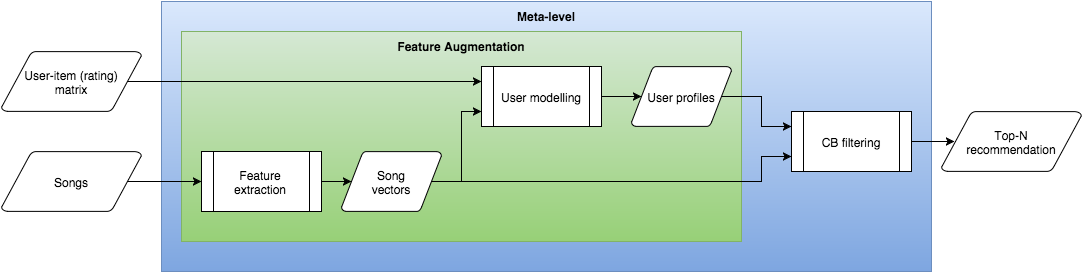
\includegraphics[width=\textwidth]{hybrid.png}
		%\caption{Diagram of the cleaning process of the Taste Profile subset}
		%\label{fig:taste_profile}
	\end{figure}
\end{frame}

\subsection{Item and user representation}
\begin{frame}
	\frametitle{Probability of music genre}
	%\begin{itemize}
		%\item Feature augmentation
		%\item Meta-level
	%\end{itemize}
	\begin{figure}[ht!]
		\centering
		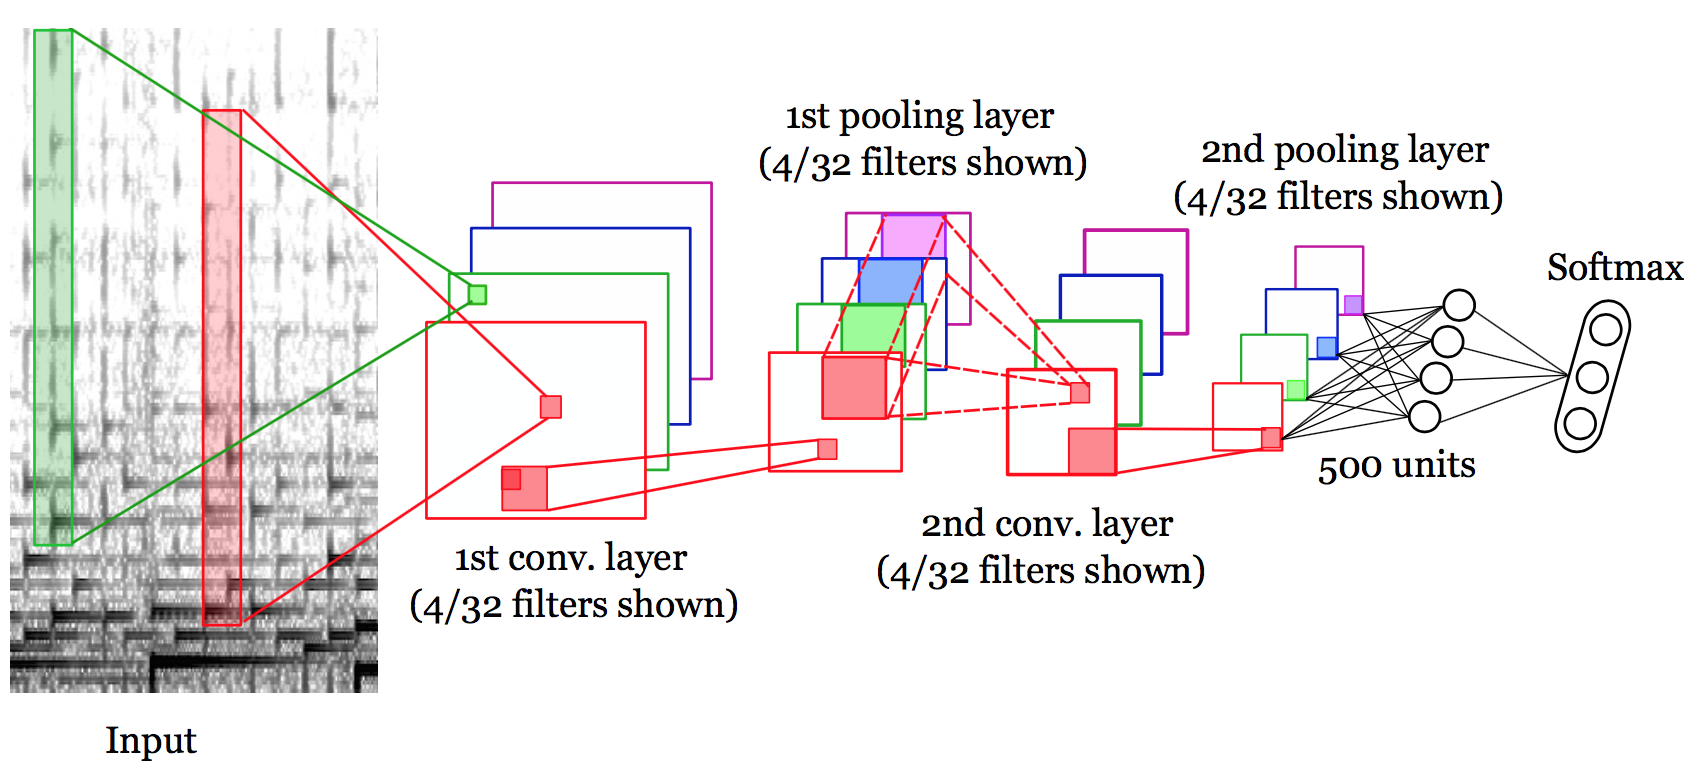
\includegraphics[width=\textwidth]{CDNN.png}
		\caption{CDNN for music genre classification (Kereliuk et al. 2015)}
		%\label{fig:taste_profile}
	\end{figure}
\end{frame}

\begin{frame}
	\frametitle{Estimation of Distribution Algorithms (EDAs)}
	\begin{figure}[ht!]
		\centering
		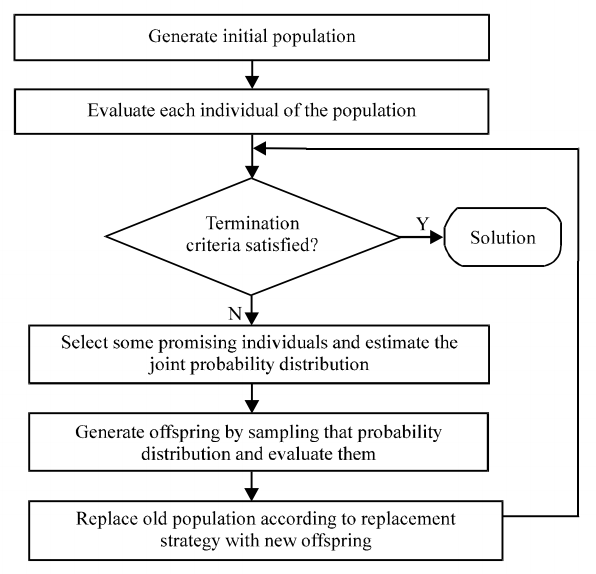
\includegraphics[width=0.5\textwidth]{eda.png}
		\caption{Flowchart for EDA (Ding et al. 2015)}
		%\label{fig:taste_profile}
	\end{figure}
\end{frame}
\begin{frame}
	\frametitle{User profile modelling}
	With permutation EDA:
	\begin{itemize}
	\item 10 tags (GTZAN) equivalent to keywords
	\item 50 weights: evenly spaced over the inverval $[0.1,\ldots,0.9]$
	\end{itemize}
	\frametitle{User profile modelling}
	With continuous EDA:
	\begin{itemize}
		\item Each genre considered as a dimension
		\item Compute mean and covariance for each dimension along individuals
		\item Sample from normal distribution
	\end{itemize}
\end{frame}

\section{Results}
\subsection{Music genre classifier}
\begin{frame}
	\frametitle{Genre classification}
\begin{table}[h!]
	\caption{Genre classification results} % title of Table
	\centering % used for centering table
	\begin{tabular}{c c c c c} % centered columns (4 columns)
		\hline\hline %inserts double horizontal lines
		Trial & Validation error (\%) & Test error (\%) & Iter. & Time elapsed (min.) \\ [0.5ex] % inserts table
		%heading
		\hline % inserts single horizontal line
		1 & 58.0 & 65.2 & 650 & 7.00 \\ % inserting body of the table
		2 & 37.6 & 46.0 & 2150 & 13.07 \\
		3 & 39.6 & 46.0 & 700 & 7.54 \\
		4 & 35.6 & 36.8 & 550 & 6.01 \\
		5 & 36.4 & 40.0 & 250 & 5.47 \\
		6 & 40.4 & 44.8 & 150 & 5.41 \\
		7 & 32.4 & 40.4 & 800 & 8.64 \\
		8 & 36.0 & 38.8 & 250 & 5.42 \\
		9 & 34.0 & 38.8 & 850 & 9.14 \\ [1ex] % [1ex] adds vertical space
		\hline %inserts single line
	\end{tabular}
	\label{table:genre} % is used to refer this table in the text
\end{table}
\end{frame}

\subsection{Hybrid recommender}
\begin{frame}
\frametitle{Top - N recommendation}
\begin{figure}[ht!]
	\centering
	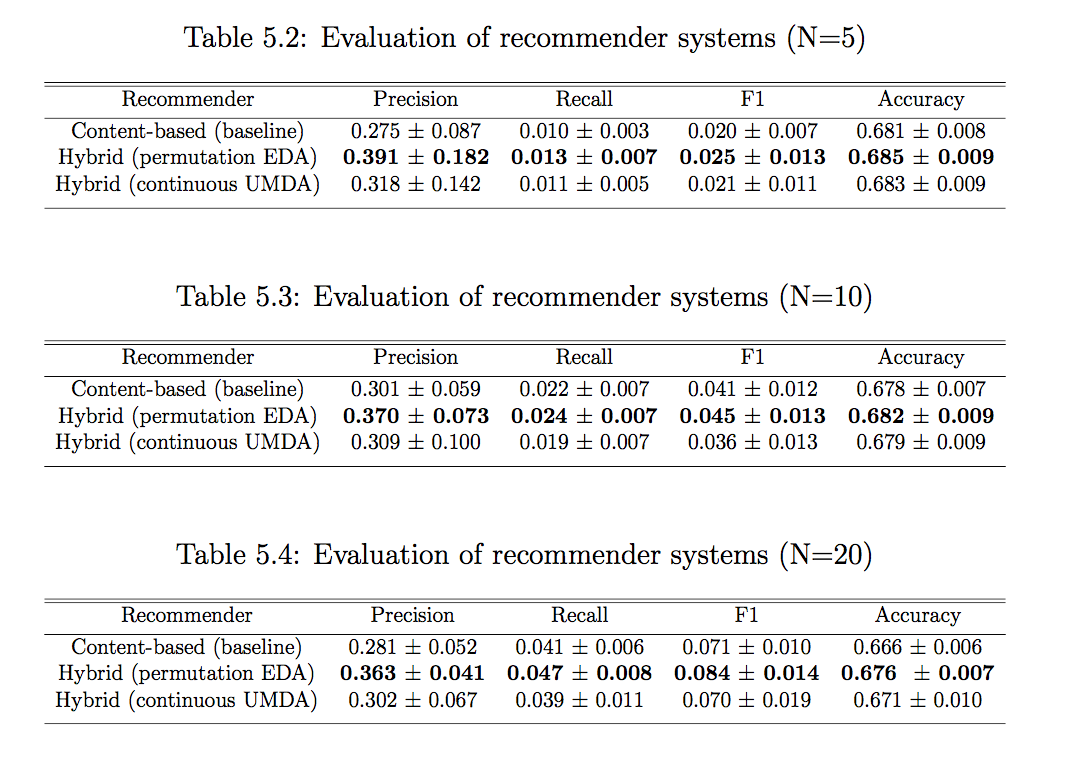
\includegraphics[width=0.9\textwidth]{a.png}
	%\caption{CDNN for music genre classification (Kereliuk et al. 2015)}
	%\label{fig:taste_profile}
\end{figure}
\end{frame}



%------------------------------------------------




\section{Conclusions and future work}
\begin{frame}
\frametitle{Conclusions and future work}
\begin{itemize}
\item CDNN produce similar results to long-established music genre classifiers
\item Hybrid permutation EDA outperforms CB
\item Investigate unsupervised deep learning
\item Online evaluation
\end{itemize}
\end{frame}



%------------------------------------------------

\begin{frame}
\Huge{\centerline{Questions?}}
\end{frame}

%----------------------------------------------------------------------------------------

\end{document} 